\documentclass[a4paper,11pt]{article}

\usepackage[utf8]{inputenc}
\usepackage[T1]{fontenc}
\usepackage[english]{babel}

\usepackage{graphicx} % Inclusion d'images
\usepackage{amsfonts} % Symboles maths
\usepackage{amsmath} % Aligner les équations
\usepackage{fullpage} % Marges
\usepackage{xspace} % Espace après macros
\usepackage{float} % Positionnement des images

\title{Robotics project}
\author{BLÉRON Alexandre \& MEYRON Jocelyn}
\date{December, 14th 2014}

\begin{document}

\maketitle

\section{Detection using stereo vision}
\subsection{Segmentation in Cartesian Space}
% Other thresholds

\subsection{Segmentation in Disparity Space}
% h_0 and p_0 => \theta and Z_0
% Compare with cartesian space

\newpage
\section{Tracking from laser scanner data}
Our state is composed of 4 parameters: the mean position and the velocity of
the region of interest. The observed measurement is the mean position (2
parameters).

The implementation is relatively straightforward: on the first frame, we know
the ROI so we can compute an initial position. We initialize our state with this
measurement. Then, for each frame, we compute the predicted value, we recenter
the ROI on this position. We finally correct the prediction by computing the
observed position (the mean position of the lidar impacts in the region of
interest).

Here are some screenshots for the tracking with a Kalman Filter. The blue cross
represents the observed position and the green cross the predicted one ($
\lambda $ is the variance of the noise during the measurement).

\begin{figure}[H]
    \centering
    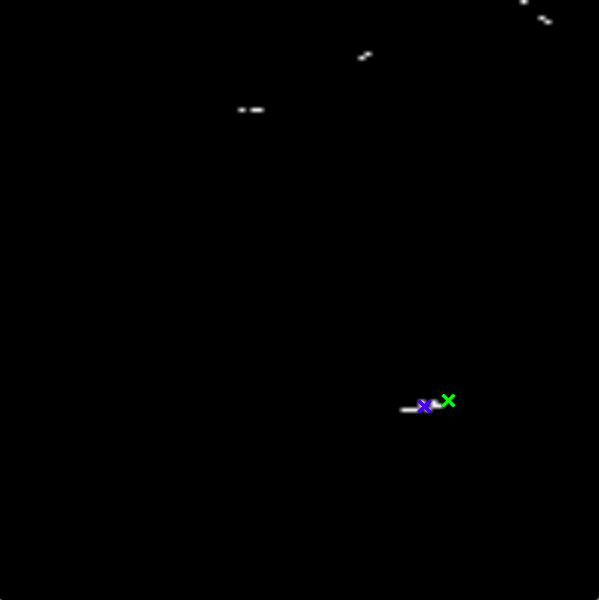
\includegraphics[scale=0.3]{pic/tracking1.png}
    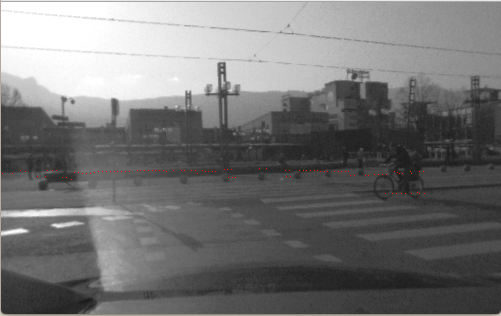
\includegraphics[scale=0.4]{pic/tracking1-left.png} \\
    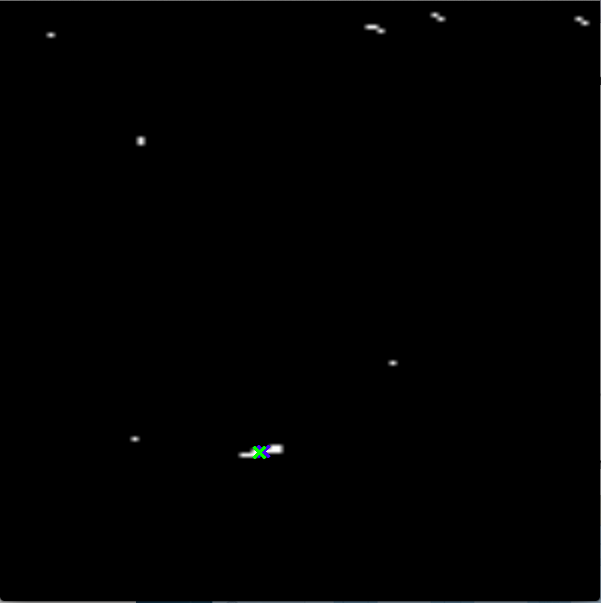
\includegraphics[scale=0.3]{pic/tracking2.png}
    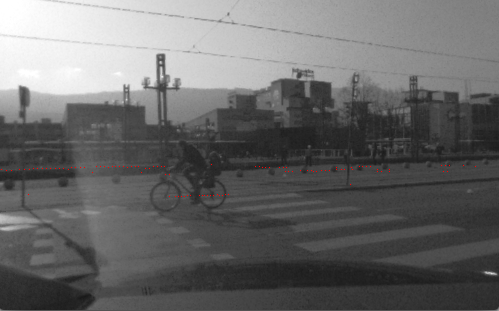
\includegraphics[scale=0.4]{pic/tracking2-left.png} \\
    \caption{Parameters: $ dt = 0.5 $ and $ \lambda = 1 $}
\end{figure}

The choice of the noise parameters is relatively important since if we choose,
for the covariance matrix of the noise, a diagonal with \og high \fg values (50
for example), then the system is not able to track the ROI anymore. More precisely,
the higher the covariance matrix is, the more difficult it is for the system to
track the bicycle: at the beginning, the prediction is very far away from the
observed one and the time for the system to be closer the target precise
increases with the value of the covariance matrix.

Using the predicted state, we can estimate the speed of the bicycle. Using
\texttt{R}, we obtain the following graph. We filtered the last 5 frames because
the bicycle was not present in the scene anymore.

\begin{figure}[H]
    \centering
    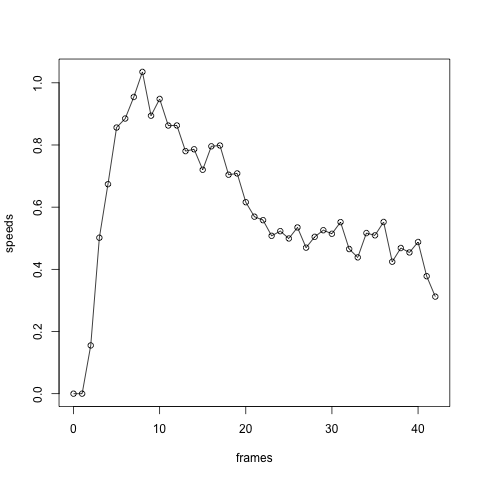
\includegraphics[scale=0.5]{pic/speed_estimation.png}
\end{figure}

The average estimated velocity is $ 0.588~m / s $ with a standard deviation of $ 0.232 $.

% Noise parameters influence?
% Estimate velocity of the target

\end{document}

